\documentclass[10pt]{article}
\usepackage{hyperref}
\usepackage[T1]{fontenc}
\usepackage[latin1]{inputenc}
%\usepackage{beton}
%\usepackage{ccfonts}
%\usepackage{concrete}
\usepackage{concmath}
\usepackage{eulervm}
\usepackage{amsmath,amsthm,amssymb}
\usepackage{mathtools}
\usepackage{multicol}
\usepackage{marginnote}
\usepackage{pgfplots}
\setlength{\parindent}{0cm}

\usepackage{comment}


\usepackage{float}
\usepackage{hyperref}
\pgfplotsset{compat=1.5}
\usepackage{graphicx}

\graphicspath{ {./images/} }
\usepackage{listings}
\usepackage{xcolor}
\definecolor{codegreen}{rgb}{0,0.6,0}
\definecolor{codegray}{rgb}{0.5,0.5,0.5}
\definecolor{codepurple}{rgb}{0.58,0,0.82}
\definecolor{backcolour}{rgb}{0.95,0.95,0.92}
\lstdefinestyle{mystyle}{
    backgroundcolor=\color{backcolour},   
    commentstyle=\color{codegreen},
    keywordstyle=\color{magenta},
    numberstyle=\tiny\color{codegray},
    stringstyle=\color{codepurple},
    basicstyle=\ttfamily\footnotesize,
    breakatwhitespace=false,         
    breaklines=true,                 
    captionpos=b,                    
    keepspaces=true,                 
    numbers=left,                    
    numbersep=5pt,                  
    showspaces=false,                
    showstringspaces=false,
    showtabs=false,                  
    tabsize=2
}

\lstset{style=mystyle}

\usepackage{mathtools}

\usepackage{wasysym}
\usepackage[margin=1.5in]{geometry} 
\usepackage{enumerate}
\index{\usepackage}\usepackage{multicol}

\usepgfplotslibrary{fillbetween}


\newcommand{\N}{\mathbf{N}}
\newcommand{\Z}{\mathbb{Z}}

\newcommand{\R}{\mathbf{R}}
\newcommand{\C}{\mathbf{C}}
\newcommand{\Pbb}{\mathbb{P}}
\newcommand{\Fcal}{\mathcal{F}}
\newcommand{\Acal}{\mathcal{A}}
\newcommand{\Ecal}{\mathcal{E}}
\newcommand{\Ebb}{\mathbb{E}}
\newcommand{\Qbb}{\mathbb{Q}}

\newenvironment{theorem}[2][Theorem]{\begin{trivlist}
  \item[\hskip \labelsep {\bfseries #1}\hskip \labelsep {\bfseries #2.}]}{\end{trivlist}}
\newenvironment{lemma}[2][Lemma]{\begin{trivlist}
  \item[\hskip \labelsep {\bfseries #1}\hskip \labelsep {\bfseries #2.}]}{\end{trivlist}}
\newenvironment{exercise}[2][Exercise]{\begin{trivlist}
  \item[\hskip \labelsep {\bfseries #1}\hskip \labelsep {\bfseries #2.}]}{\end{trivlist}}
\newenvironment{reflection}[2][Reflection]{\begin{trivlist}
  \item[\hskip \labelsep {\bfseries #1}\hskip \labelsep {\bfseries #2.}]}{\end{trivlist}}
\newenvironment{proposition}[2][Proposition]{\begin{trivlist}
  \item[\hskip \labelsep {\bfseries #1}\hskip \labelsep {\bfseries #2.}]}{\end{trivlist}}
\newenvironment{corollary}[2][Corollary]{\begin{trivlist}
  \item[\hskip \labelsep {\bfseries #1}\hskip \labelsep {\bfseries #2.}]}{\end{trivlist}}

\newenvironment{definition}[2][Definition]{\begin{trivlist}
  \item[\hskip \labelsep {\bfseries #1}\hskip \labelsep {\bfseries #2.}]}{\end{trivlist}}

\begin{document}
	
  \renewcommand{\qedsymbol}{\smiley}
	\title{Optimal Decision Making \\ Report}
	\author{Aurelien Balice-Debbas, Marijn van der Meer, Hugo Bassas}
	
	\maketitle

\section{Mean Absolute Error Penalised Regression}

\begin{figure}[!ht]
  \centering
  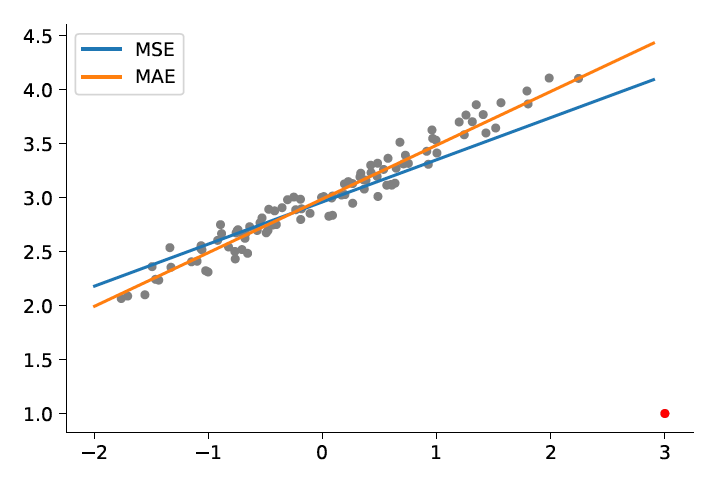
\includegraphics[width=0.5\textwidth]{doc/images/im1_.png}
  \caption{MSE vs. MAE estimators for a dataset with 1 outlier (red dot). }
  \vspace{-3mm}
  \label{fig:mae-mse}
\end{figure}

  \begin{exercise}{1} 
  (5 points).
  Figure~\ref{fig:mae-mse} visualises the outputs predicted by the MSE
and MAE estimators on a dataset with 1 outlier. Explain the difference between the two estimators intuitively. Hint: Compare how Eq.~\ref{eq:mse} and Eq.~\ref{eq:mae} penalise errors. 

\begin{equation}\label{eq:mse}
    \hat\theta_{MSE} = \text{arg min}_\theta \frac{1}{N} \sum_{i=1}^N(y^{(i)}-\theta^Tx^{(i)})^2
\end{equation}

\begin{equation}\label{eq:mae}
    \hat\theta_{MAE} = \text{arg min}_\theta  \frac{1}{N} \sum_{i=1}^N|y^{(i)}-\theta^Tx^{(i)}|
\end{equation}


\textit{Answer.} The MSE estimator is computed from the sum of squared distances between our target variables $y^{(i)}$ and predicted values $\hat y^{(i)} = \theta^Tx^{(i)}$ while MAE uses the sum of absolute differences i.e., the average magnitudes of errors. MSE is more easy to use in optimisation problems because it is convex while MAE is not and has the same gradient everywhere. But MAE is more robust to outliers as can be seen in Fig.~\ref{fig:mae-mse}. This is due to the fact that MSE squares errors, and thus for an outlier we have that $e^2 >> |e|$. When searching for optimal weights $\hat\theta$, MSE will have a tendency to try to adjust in a way of minimising big errors such as the one outlier in our case. In our case, this explains why the model predicted using MSE (in blue) is closer to the outlier than the one from MAE (in red). 
  \end{exercise}

\begin{exercise}{2.1}
(5 points) In case of high-dimensional inputs (d > N), it makes sense to seek a sparse
parameter vector $\theta$. This means that many components of $\theta$ should be zero. The non-zero components of $\theta$ then correspond to the key features or key inputs that have a significant impact on the outputs. Sparsity can be induced by adding an L1-penalty to the objective function of Eq.~\ref{eq:mse} or Eq.~\ref{eq:mae}, which yields the least absolute
shrinkage and selection operator (LASSO) method of regression analysis. In case of the MAE objective, the resulting LASSO estimator satisfies:
\begin{equation}\label{eq:lasso}
    \hat\theta_{lasso} = \text{arg min}_\theta  \frac{1}{N} \sum_{i=1}^N|y^{(i)}-\theta^Tx^{(i)}| + \lambda ||\theta||_1 
\end{equation}
In practice, $\lambda$ is a hyperparameter typically chosen by cross validation. That is, we randomly partition D into a training dataset $D_{train}$
and a validation dataset $D_{val}$. We then solve Eq.~\ref{eq:lasso} using only $D_{train}$ for different
values of $\lambda$ and select the estimator that has minimal MAE on $D_{val}$. Rewrite Eq.~\ref{eq:lasso} as a linear program (not necessarily in standard form).

\textit{Answer.} 
We write $\Lambda = [\lambda_1, ... , \lambda_k]$ the set of all values for the hyperparameter $\lambda$. We also note $x_i\in \mathbb{R}^d \; \forall i=1 ,\dots, N$ the data samples and $y_i\in \mathbb{R}$ the target variable for input $x_i$. For $\lambda\geq 0$, LASSO regression finds and optimal $\theta \in \mathbb{R}^d$ such that   

\begin{equation}
 \displaystyle\sum\limits_{i=1}^{N}  |y_i-\theta^Tx_i| + \lambda\displaystyle\sum\limits_{i=1}^{d}|\theta_i|
\end{equation}

is minimal. 

With the addition of auxiliary variables $z_i$ and $\delta_i$, we use the fact that $|y_i - \theta^T x_i| < z_i$ is equivalent to $-z_i < y_i - \theta^T x_i  < z_i$. So, minimising the sum of $ |y_i-\theta^Tx_i|$ is equal to minimising the sum of $z_i$ because

\begin{equation*}
    \sum\limits_{i=1}^{N}  |y_i-\theta^Tx_i| < \sum\limits_{i=1}^{N} z_i
\end{equation*} 

The same applies to $|\theta_i|, \delta_i$. So, we can write the following linear program:
\begin{equation*}
\begin{array}{lll@{}lll}
&\text{min}  &\displaystyle\sum\limits_{i=1}^{N}z_i +  \lambda\sum\limits_{i=1}^{d}\delta_i &\\
\text{subject to} 
&& y_i-\theta^Tx_i &\leq z_i && i=1 ,\dots, N \\
&& -y_i+\theta^Tx_i &\leq z_i && i=1 ,\dots, N \\
                 && \theta_i &\leq \delta_i &&  i=1 ,\dots, d \\
                && -\theta_i &\leq \delta_i &&  i=1 ,\dots, d 
\end{array}
\end{equation*}
To rewrite this in standard form we introduce slack variables $s,t,u,v$: 
\begin{equation*}
\begin{array}{lll@{}lll}
&\text{min}  &\displaystyle\sum\limits_{i=1}^{N}z_i +  \lambda\sum\limits_{i=1}^{d}\delta_i &\\
\text{subject to} 
&& -\theta^Tx_i - z_i + s &= y_i && i=1 ,\dots, N \\
&& +\theta^Tx_i -z_i + t &= y_i && i=1 ,\dots, N \\
                 && \theta_i - \delta_i + u&= 0  &&  i=1 ,\dots, d \\
                && -\theta_i - \delta_i + v &= 0  &&  i=1 ,\dots, d 
                \\
                && s,t,u,v &\geq 0  && 
\end{array}
\end{equation*}
\end{exercise}

\begin{exercise}{2.2}
(5 points)
Compute
the MAE of the resulting estimator on the separate test sets provided on
Moodle. Compare the test performance against the training performance. 

\textit{Answer}. 
\begin{enumerate}
    \item Training MAE: $44.7337$
    \item Test MAE: $45.4309$
\end{enumerate}
We see that the performance on both sets are very close, though the result on the test set is slightly larger, which is to be expected as the model was trained on the other set.
\end{exercise}

\begin{exercise}{2.3}
(5 points)
Use cross-validation to tune the hyperparameter. Compare again the test performance against the training performance.

\textit{Answer}. 
The optimal parameter $\lambda$ was chosen as the one yielding the smallest loss on the test set (Figure~\ref{fig:hyperpar}). 
\begin{enumerate}
\item Optimal $\lambda$: $1e-5$ 
\item Optimal value: $14049.7677$
    \item Training MAE: $42.4461$
    \item Test MAE: $46.4249$
\end{enumerate}
Again, performance on both sets are very close, though the result on the test set is slightly larger.

\begin{figure}[!ht]
  \centering
  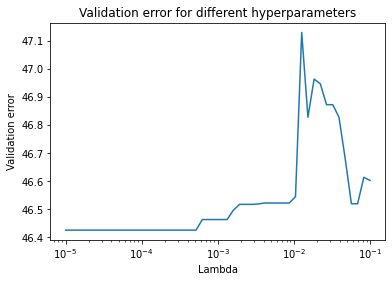
\includegraphics[width=0.5\textwidth]{doc/images/download (14).png}
  \caption{Validation error for different hyperparameters $\lambda_$.}
  \vspace{-3mm}
  \label{fig:hyperpar}
\end{figure}


\end{exercise}


\section{Convex Hulls}
\begin{exercise}{3}

(5 points). Denote by $X$ the feasible set of Eq.~\ref{eq:lp-2}. Write the
convex hull of $X$ using a finite set of simple (in-)equalities on $x_1$ and $x_2$ and find its vertices. Plot both $X$ and $conv(X)$.

\begin{equation}\label{eq:lp-2}
\begin{array}{ll@{}ll}
\text{min}  &-x_1 - 2x_2\\
\text{subject to} 
& x_1+x_2 &\leq 1 \\
&x_1,x_2 &\in \{0,1\}
\end{array}
\end{equation}

\textit{Answer.}
Le $X$ be the feasible set of Eq.~\ref{eq:lp-2}, the convex hull $conv(X)$ can be written as: 
\begin{equation}\label{eq:convex-hull}
\begin{array}{l@{}ll}
 x_1 + x_2 &\leq 1 \\
 x_1,x_2  &\geq 0 \\ 
 \end{array}
\end{equation}
The vertices of $conv(X)$ are $(0, 0)$, $(0, 1)$ and $(1, 0 )$. Figure~\ref{fig:hull} shows the feasible set $X$ and its convex hull $conv(X)$.

\begin{figure}[!ht]
  \centering


\begin{tikzpicture}
\begin{axis}[
   % title={Temperature dependence of CuSO$_4\cdot$5H$_2$O solubility},
    xlabel={$x_1$},
    ylabel={$x_2$},
    xmin=-0.5, xmax=1.5,
    ymin=-0.5, ymax=1.5,
    xtick={0,0.5, 1, 1.5},
    ytick={0,0.5, 1, 1.5},
    legend pos=north west,
    ymajorgrids=true,
    grid style=dashed,
    axis lines = middle,
]
    \addplot [thick,color=blue,mark=o,fill=blue, 
          fill opacity=0.05]coordinates {
            (0, 0) 
            (0, 1)
            (1, 0)  };
    \addplot[name path=f,domain=0:1,blue] {1 - x};
    \addplot[name path=f2,domain=0:1,blue] {0};
    \path[name path=axis] (axis cs:0,0) -- (axis cs:1,0);
    \addplot [
        thick,
        color=blue,
        fill=blue, 
        fill opacity=0.05
    ]
    fill between[
        of=f and axis,
        soft clip={domain=0:1},
    ];
\end{axis}
\end{tikzpicture}

 \caption{Plot of feasible set $X$ (coordinates $(0, 0)$, $(0, 1)$ and $(1, 0 )$) and its convex hull $Conv(X)$ (lines in dark blue)}
  \vspace{-3mm}
  \label{fig:hull}
\end{figure}

\end{exercise}

\begin{exercise}{4}
(5 points). Replace the feasible set of Eq.~\ref{eq:convex-hull} with its convex hull and solve the resulting linear program using Python. Report the optimal decision variables. Explain why they must be binary. Hint:
Characterise the BFS of the convex hull of the feasible set.


\textit{Answer.}
Using the convex hull, we get the following linear program : 

\begin{equation*}
\begin{array}{lll@{}lll}
&\text{min}  & - x_1 - 2 x_2  &\\
\text{subject to} 
&& x_1 + x_2 \leq 1 \\
&&  x_1  \geq 0,  x_2 \geq 0 \\
          
\end{array}
\end{equation*}

This transforms our Integer LP from before into a standard LP. Solving the new LP with Python, we obtain  the following optimal vertex: $x_1^*=  0.0$ and $x_2^* = 1.0$. So, the extreme points of $conv(X)$ have integer coordinates and are indeed binary. In the lecture, we saw that MILP can be solved by finding an extreme point solution to CMILP which is what has been done here. We saw that this was because the extreme points of $conv(X)$ have integer coordinate and they must be binary because of the original feasible set $X$. If the solution using  

\textbf{COMPLETER AVEC BFS}

%Let $x^{\*}$ be an extreme point %% Ore BSF, need to check 
%Suppose towards contradiction that there exist a BFS $x^*$ that is not binary. So that exists $x_i^*$ s.t $0< x_i^* < 1 $ 
%We want to define $y$ and $z$ so they are feasible solutions and $x^* = \frac{1}{2} (y + z) $ which contradicts the fact that $x^* $ is an extreme point. 
\end{exercise}
  
  
\section{Zero-Sum Games}
\begin{exercise}{5.1}
(3 points) Characterise your decisions variables and feasible set.

\textit{Answer.}
The only decision attributed to the player i.e., the one who is trying to save their money is how much money to put in each hiding spot $x_i$. That amount $x_i$ is subject to two different constraints:
\begin{itemize}
    \item The amount of money $x_i$ in hiding spot $i\in[I]$ cannot exceed the maximum capacity $C_i$ of money that can be hidden in this spot and has to be non negative.
    \item The total amount of money hidden in all spots must be equal to the total amount of money the player has $C$ (in our case \$10,000). This is assuming the player wants to hide all their money. 
\end{itemize}

To summarise this, the constraints delimiting the player's feasible set can be expressed as:

\begin{equation}\label{eq:owner}
\begin{array}{ll@{}lll}

\displaystyle\sum\limits_{i=1}^{I} x_i = 10'000 \\ \\
x_i \leq C_i && i=1 ,\dots, I\\ 
x_i \geq 0 && i=1 ,\dots, I
\end{array}
\end{equation}
\end{exercise}

\begin{exercise}{5.2} (3 points) 
Characterise the thief's decision variables and feasible set.

\textit{Answer.}
The two decision variables attributed to the adversary, in this case the robber is how much time they put into searching for money, and where to spend this time. However, since these two variables are redundant, they can be condensed into one, which is the time spent searching for money in spot $i$, represented by the variable $z_i$. This time is subject to two constraints:

\begin{itemize}
    \item The total amount of time spent searching cannot exceed the time \textit{T} needed for the police to arrive at the house.
    \item The time spent in one spot multiplied by the area's search difficulty factor $p_i$ cannot exceed 1. If it equals 1, it means all of the money in that spot has been found.
\end{itemize}

So, the constraints delimiting the thief's feasible set can be expressed as

\begin{equation}\label{eq:thief}
\begin{array}{ll@{}lll}

\displaystyle\sum\limits_{i=1}^{I} z_i \leq T \\ \\
z_i p_i \leq 1 && i=1 ,\dots, I\\ \\
z_i \geq 0
\end{array}
\end{equation}
\end{exercise}

\begin{exercise}{5.3} (3 points) Use the solutions of the first two questions to formulate a MinMax problem with objective function $f(x, z) =\sum\limits_{i=1}^{I} x_i z_i p_i $. 

\textit{Answer.}
The problem can be written as the following:

\begin{equation}
\begin{array}{ll@{}llll}
\displaystyle\min_{x}\displaystyle\max_{z} & \displaystyle\sum\limits_{i=1}^{I} x_i z_i p_i\\
\text{subject to} 
& \displaystyle\sum\limits_{i=1}^{I} x_i = C\\
& \displaystyle\sum\limits_{i=1}^{I} z_i \leq T \\
& x_i \leq C_i \\
& z_i p_i \leq 1 &&i=1 ,\dots, I\\
                & x_i,z_i \geq 0 &&i=1 ,\dots, I
\end{array}
\end{equation}

\end{exercise}

\begin{exercise}{5.4} (8 points)
Dualise the inner maximisation problem to reformulate the MinMax problem as a standard minimisation problem, which can be addressed with linear programming solvers. Hint: The decision variables of the outer minimisation problem represent constants for the inner maximisation problem.

\textit{Answer.}
Assuming that we keep the outer minimisation constant while resolving the inner maximisation problem, we can keep x constant. Thus, we can reformulate the maximisation as follows:

\begin{equation}
\begin{array}{ll@{}lll}
\displaystyle\max_{z} && \displaystyle\sum\limits_{i=1}^{I} x_ip_iz_i\\

\text{subject to} 
&& \displaystyle\sum\limits_{i=1}^{I} z_i \leq T &&  \\
                && z_i  \leq p_i  &&  i=1 ,\dots, I\\
                && z_i\ \geq 0 &&i=1 ,\dots, I\\ 

\end{array}
\end{equation}

The problem becomes a maximisation problem centered on the variables $z_i$, which is the time allocated by the thief to searching each spot $i$. We write $y_i$ as its primal variable. The problem can be dualised as follows. 
We apply the formula that the dual (D) of the primal problem (P): 
\begin{equation}
\begin{array}{lll@{}llllll}
\text{(P)}  &\displaystyle\min_{y}\ &c^Ty && \text{(D)} & \displaystyle\max_{z}\ &b^Tz\\
&\text{subject to} 
&Ay\geq b &&&\text{subject to} &A^Tz\leq c\\
&& y\ \geq 0 &&&&z\ \geq 0\\ 

\end{array}
\end{equation}
In our case, we see that we actually start from the dual formulation and would like the primal problem. So, we write $z_i\in\mathbb{R}^{I}$ as our dual variable and $b^T = \begin{pmatrix}x_1p_1 & x_2p_2 & ... &x_Ip_I\end{pmatrix} \in\mathbb{R}^{I}$. Then  $c^T = \begin{pmatrix}T & p_1 & ... &p_I\end{pmatrix}\in\mathbb{R}^{I+1}$ and
\begin{equation*}
    A^T \in\mathbb{R}^{I+1xI} = \begin{pmatrix}
1 & 1 & ... & 1\\
1 & 0 & ... & 0 \\
0 & 1 & ... & 0 \\
0 & 0& ... & 1
\end{pmatrix}
\end{equation*}

where the first row of $A^T$ are only $1$. From this, we can write the primal formulation:

\begin{equation}
\begin{array}{lll@{}lll}
(P) &\displaystyle\min_{y}\ &&Ty_{I+1} + \displaystyle\sum\limits_{i=1}^{I} \frac{1}{p_i}y_i\\

&\text{subject to} 
&& y_{I+1} + y_{i+1}\geq x_ip_i  &&  i=1 ,\dots, I\\
&&& y_i\ \geq 0 && i=1 ,\dots, I+1\\ 

\end{array}
\end{equation}

We notice that there is an extra variable $y_{I+1}$ in the minimisation problem. This variable refers to the total amount of money the thief gets, regardless of his strategy.
From weak duality, we know that $OPT_{dual}\leq OPT_{primal}$ and so the primal problem we found here gives an upper bound on the optimal time the thief takes per spot ($z_i^*$). Should the problem be implemented correctly, then in the optimal solution all the y variables should be equal to zero and $y_{I+1}$ should be non-zero.\\




\end{exercise}

\begin{exercise}{5.5} (3 points) Implement the resulting linear program in Python and solve it for the provided input data $p, C \in \mathbb{R}^I$ and $T \in \mathbb{R}$. Report the worst amount of money you lose, the optimal plan for hiding the money and the thief's optimal search strategy. 

\textit{Answer.}
Upon implementing the modified problem, we get the following results:

\begin{equation}
\begin{array}{ll@{}lll}
x = \begin{pmatrix}
2000\\
1000\\
1961.0894\\
1634.2412\\
1225.6809\\
2178.9883\\
\end{pmatrix} 
\approx 
\begin{pmatrix}
2000\\
1000\\
1961.09\\
1634.24\\
1225.68\\
2178.98\\
\end{pmatrix}

\\ \\

y_{I+1} = 1961.0894 \approx 1961.09
\end{array}
\end{equation}
Furthermore, the other $y_i$ are indeed zero. As we can see, the value found by the dual problem is the same as the value of the money hidden in the third spot. This spot is also one of the two spots (along with spot 2) which can be searched in its entirety by the thief within the allocated time T without being caught by the police. Further analysis of this solution can show that searching a combination of these hiding spots still yields a maximum profit of 1961.08 dollars for the thief. For example, should the thief search the 5th spot completely and the last spot until time runs out, he would still end up with less than or equal to 1961.08 dollars.

The optimal strategy for the thief would be to search position 3 completely (that is, until time runs out) to get the maximum amount of money.




\end{exercise}

  
 \section{Adversarial Training}
  \begin{exercise}{6}
  Write the convex hull of the adversary's feasible set 
  \begin{equation}
      Z  =\Bigg \{ z\in \mathbb{R}^N: \sum_{i=1}^{N}z_i = k, z_i \in \{0,1\} \;\forall i\in[N]\Bigg \}
  \end{equation}
  
  using a finite set of (in-)equalities on $z_i$. Note that k is an integer. Explain why your formulation is indeed the convex hull.

  \textit{Answer:} First of all, we notice that all feasible points (and thus the convex hull) must be in the positive quadrant of $\mathbb{R}^N$ due to the coordinates of $z$ being $z_i \in \{0,1\}$. Furthermore, in the extreme case when $k=N$ then the only feasible point is $z_i = 1^N\in\mathbb{R}^N$ (the vector that is one everywhere). So, in the case of $k=N$, the convex hull is just the point itself (convex by definition). Another special case is when $k=1$ and the vectors $z$ are just the unit vectors $e_i \in\mathbb{R}^N$. In that case, the convex hull is given by the shape delimited by the unit vectors (a line in 2D and a triangle in 3D, Fig.~\ref{fig:convex-hull}). 
  
 \begin{figure}[!ht]
  \centering
  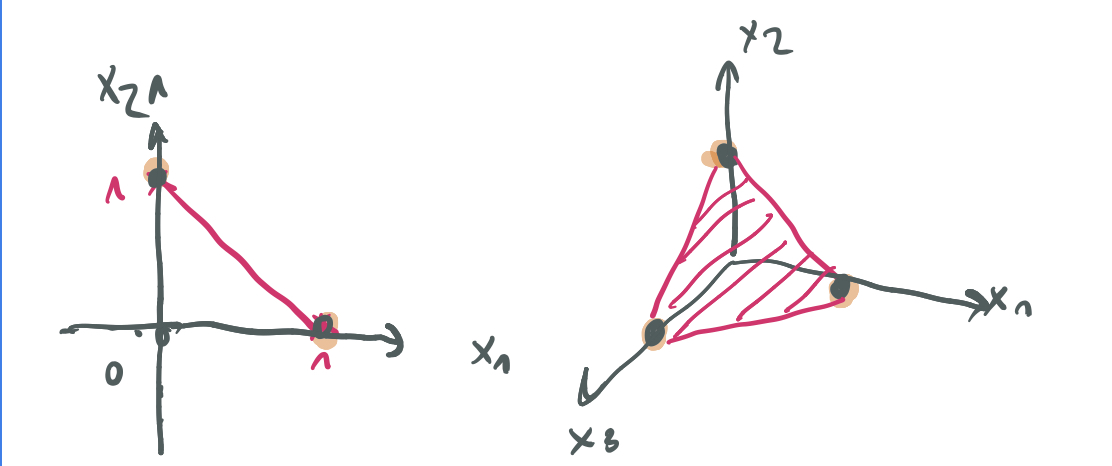
\includegraphics[width=0.5\textwidth]{doc/images/IMG_0038.jpg}
  \caption{Figure 1: Convex hull of feasible set in 2D and 3D in the case where $k=1$.}
  \vspace{-3mm}
  \label{fig:convex-hull}
\end{figure}
 
 For the more general case, we first note that, due to the combinatorial properties of the solutions $z\in\mathbb{R}^N$, the set of feasible solutions is finite i.e., because $z$ have to satisfy $\sum_{i=1}^{N}z_i = k$, there is only a finite number of possibilities assuming $N$ is finite. By Weyl's theorem~\cite{rockafellar1970convex}\cite{QUEYRANNE19921}, the convex hull of $Z$ is a convex polyhedron and can thus be defined by a finite set of linear inequalities.
 
 We define the convex hull by $conv(Z)= \{ z \in\mathbb{R}^N | Az\leq b, z_i \geq 0 \}$ where $A \in\mathbb{R}^{2xN} = \begin{pmatrix}
1 & 1 & ... & 1\\
-1 & 1 & ... & -1
\end{pmatrix}$ and $ b = \begin{pmatrix}k\\-k
\end{pmatrix}$. So, the vertices of the convex hull are the extreme points of the feasible set of the Integer Linear Problem ILP:

\begin{equation}
\begin{array}{l@{}llll}
&&\text{min}_\theta F(\theta, z)\\
\text{subject to} 
&& \displaystyle\sum_{i=1}^{N}z_i &\leq k & i=1 ,\dots, N \\
&& -\displaystyle\sum_{i=1}^{N}z_i &\leq -k & i=1 ,\dots, N  \\
&& z_i \in \{0,1\} && i=1 ,\dots, N 
\end{array}
\end{equation}
where $F(\theta, z) = max_{z_1, ...z_N} \displaystyle\frac{1}{k} \sum_{i=1}^{N}z_i|y^i-\theta^Tx^i|+\lambda || \theta||_1$. 
The convex hull as defined above has a finite number of constraints because its bounded by the number of constraints in the ILP, which is finite. The hull is convex by definition of the feasible region. 


Notes:
- linear integer program (LIP), an optimal integer solution is also optimal over the
convex hull of all integer feasible solutions,

 \end{exercise}
 
 
\begin{exercise}{7}

\begin{enumerate}
    \item 

We want to transform the following Min-Max problem. 

\begin{equation*}
\begin{array}{lll@{}lll}
\min\limits_{\theta}&\max\limits_{z_1,...,z_N}  &\frac{1}{k}\displaystyle\sum\limits_{i=1}^{N}z_i|y^{(i)} - \theta^\top x^{(i)}| +  \lambda||\theta||_1 &\\
\text{subject to} 
&& \displaystyle\sum\limits_{i=1}^{N}z_i = k  && \\
                \\
                && z_i \in  \{ 0, 1 \}   & \forall i \in [ N ]& 
\end{array}
\end{equation*}


First, using the solution from Question 3, lets write the dual of the inner minimization problem using the same logic : 


\begin{equation*}
\begin{array}{lll@{}lll}
&\max\limits_{z_1,...,z_N}  &\frac{1}{k}\displaystyle\sum\limits_{i=1}^{N}z_i|y^{(i)} - \theta^\top x^{(i)}| +  \lambda||\theta||_1 &\\
\text{subject to} 
&& \displaystyle\sum\limits_{i=1}^{N}z_i = k  &&  \\
                \\
                && z_i \in  \{ 0, 1 \}   & \forall i \in [ N ]& 
\end{array}
\end{equation*}

With $p_i$  replaced by $ 1 / k$ and $T$ replaced by $k$ making  $\beta_i$  unconstrained and changing the order of the constraint inequality because of the equality in the maximisation problem  . 

The maximization problem is transformed into : 

\begin{equation*}
\begin{array}{lll@{}lll}
&\min\limits_{y}   &  k\beta_{N + 1 }  + \sum\limits_{i=1}^{N}\beta_i  + \lambda||\theta||_1  &\\
\text{subject to} 

&&  \beta_{N + 1 } + \beta_i   & \geq \frac{1}{k}|y^{(i)} - \theta^\top x^{(i)}| &  i=1 ,\dots, N \\
                \\
                && y_i    &  \geq 0 % unconstrained& %% ?? Really unconstrained ? 
\end{array}
\end{equation*}

We then assigning $\beta_{N+1} = \alpha$, and as in Exercice 2, we use the fact that $|y_i - \theta^T x_i| \leq \beta_i$ is equivalent to $-\beta_i + \alpha < y_i - \theta^T x_i  < \beta_i + \alpha$ to rewrite the full linear program. 

We also use the same principle for $|\theta_i|$ using $b_i$ as an auxiliary variable. 

Finally, we obtain the following program : 

\begin{equation*}
\begin{array}{lll@{}lll}
 \min\limits_{\theta, b_i} &\min\limits_{\beta. \alpha}   &  k\alpha  + \sum\limits_{i=1}^{N}\beta_i  + \lambda\sum\limits_{i=1}^{d} b_i   &\\
\text{subject to} 

&&  \alpha + \beta_i    & \geq \frac{ y^{(i)} - \theta^\top x^{(i)}}{k}&  i=1 ,\dots, N \\
&&  \alpha + \beta_i    & \geq \frac{- y^{(i)} + \theta^\top x^{(i)}}{k} &  i=1 ,\dots, N \\
                \\
                && \beta_i    & \geq 0  & \\ %% ?? Really unconstrained ? 
                && - b_j \leq \theta_j \leq b_j & & j = 1 \dots, d
\end{array}
\end{equation*}

Merging the two minimization we obtain the desired result. 



\item \textit{Implement the linear program (8) in MATLAB or Python using the skeleton code we provide on Moodle and solve it for 50 logarithmically spaced values of in the interval. For each of these values compute the MAE of the corresponding estimator on the validation set, and select the best robust estimator. To assess the beneffts of robust cross validation over standard cross validation, compare the MAE of the robust estimator against the MEA of the estimator found in Question 2.3. In both cases the MEA should be computed on the test set.}




\item \textit{For the robust estimator found above, compare also the MEA on the test set against the MEA on the training set. Is there a significant difference to what you observed in Question 2.3.? Interpret your observations?}


We notice a significant difference between the MEA on the test set against the the Training Set. In this adversarial training procedure, we force the outliers to be in the training set.  Thus, it is logical that the MAE of the trainig set is larger than that of the test set. In the previous question, the outliers were evenly distributed between the training and the test, and the model was therefore less robust. 


\end{enumerate}

 \end{exercise}

  \section*{Appendix}
\newpage  
 \begin{thebibliography}{9}
\bibitem{rockafellar1970convex} 
Rockafellar, R Tyrrell: Convex analysis, 1970, volume 36, Princeton university press
\bibitem{QUEYRANNE19921} 
M. Queyranne and Y. Wang: On the convex hull of feasible solutions to certain combinatorial problems, 1992, volume 11, Operations Research Letters
\\\texttt{https://www.sciencedirect.com/science/article/pii/0167637792900558}
\end{thebibliography}
 
\end{document}

